\chapter{Entropy and Fractal Dimension Approach}
\textit{by Florian Fallenbüchel}\\
This chapter will explain our approach on the classification of the
genre via the entropy and fractal dimension of the song. This approach
is interesting, because it does not consider musical information such as
harmony, melody, beat and tempo, heavily reducing the size of the data
to be processed during training. The entropy is a measure of the
disorder of the signal, indicating the quantity of change of the signal
energy between consecutive parts of the track. The fractal dimension is
a measure of the complexity of the signal, as it indicates the ratio of
the change of detail to the change in scale at which the detail is
measured. This term is mostly used in fractal geometry, as fractals have
infinite lengths between any two points, making them more complex than
their topological dimension, but less complex than the next higher one.
This interdimensionality is given by the fractal dimension.\\

\section{Method}
We follow the work of Goulart \textit{et al.}~\cite{entropy} from 2012,
who used the entropy approach together with combined support vector
machines. They achieved 100\% classification accuracy on a set of 90
songs equally distributed over 3 different genres, with 80-90\% of the
data used for training. We try to extend this method to a larger amount
of classes, combining it with neural networks for classification.\\
For the calculation of the entropy, we need the energy approach of
signal theory, as presented in Elements of Information Theory
\cite{infotheo} by Cover and Thomas. The song is divided into frames of
1024 samples with 50\% overlap between consecutive frames and the
entropy $E$ then is defined as
\begin{equation}
	E = - \sum_{i=0}^{1023} p_{i} \log_{2}(p_{i}),
\end{equation}
with $p_{i}$ being the proportion of the sample energy to the
energy of the whole frame
\begin{equation}
	p_i = \frac{y_i}{\sum_{j=0}^{1023} y_j}.
\end{equation}
\\
\noindent From the now obtained set of entropies of the song we
calculate five features, namely the average entropy, the standard
deviation of the entropies, the maximum and minimum entropy and the
absolute maximum difference of entropies between consecutive frames.
Those are the first five entries of our input vector for the neural
network.\\
For the calculation of the fractal dimension they suggest a box counting
algorithm. The basic principle of these algorithms is to calculate the
number of boxes of different sizes necessary to cover the entire signal.
After that, a linear least squares solution is computed on the logarithm
of the number of boxes and the inverse logarithm of the respective box
size ($\frac{1}{log(boxs)}$). The slope of the resulting curve then
resembles the fractal dimension.\\
For the implementation of the algorithm, we needed to improvise, because
the box counting algorithm Goulart \textit{et al.} used in their work is
described in the book ``Fractal Speech Processin''~\cite{fractal} by
Al-Akaidi, which is not purchasable or accessible through online
libraries at the moment. We therefore adopted the box counting algorithm
presented by Boshoff~\cite{boxcount}, as it promises fast computation
time due to the doubling of the box size during each step. The fractal
dimension is the last element of our input, resulting in a six
dimensional input vector for the neural network. We vectorized all
algorithms, to be able to efficiently process the huge amount of
available data in a short amount of time.

\section{Model}
As our input data is relatively simple, we can use a conservative
implementation of a neural network for the classification, without the
need for convolutions. Figure~\ref{entropymodel} shows the architecture
of our naive network design. Our hidden layers are of size 1024 and we
chose parameterized ReLUs with a parameter for every connection, as well
as batch normalization and dropout for every layer. Batch normalization
accellerates training, as it reduces the amount by what the hidden unit
values shift around, normalizing the input from previous layers to a
common scale. The dropout layers should stabilize the prediction
accuracy by eliminating parts of the information during training,
reinforcing the remaining neurons.

\begin{figure}
	\centering
	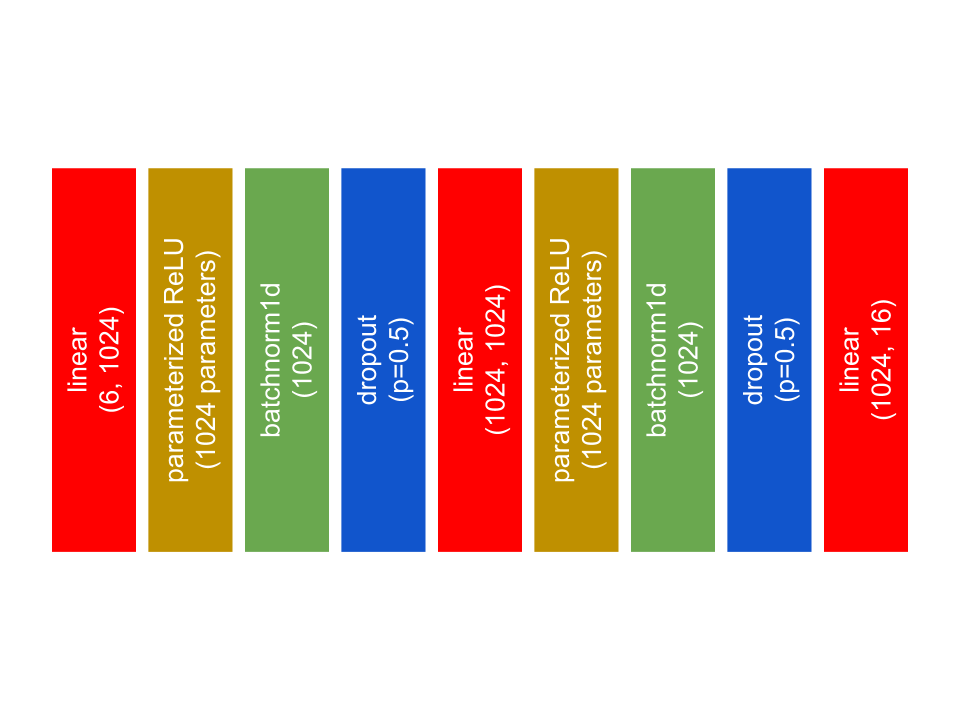
\includegraphics[width=0.65\textwidth]{images/entropymodel.png}
	\caption{Architecture of the neural network used for the classification
	of the 6-dimensional entropy-fractal vector to one of the 16 top
	genres from the dataset.}
	\label{entropymodel}
\end{figure}

\section{Training}
For the training, we used a maximum of 180 seconds per song, as processing
the full length of every track would have taken several days on our
available hardware.

\begin{center}
	\begin{tabular}{ p{0.25\textwidth} p{0.2\textwidth} p{0.2\textwidth} p{0.2\textwidth}}
		Genre & Accuracy & Hits & from Total\\
		\hline
		Instrumental & $0.00\%$ & 0 & 430\\
		Folk & $0.00\%$ & 0 & 558\\
		Country & $0.00\%$ & 0 & 37\\
		Pop & $0.00\%$ & 0 & 481\\
		Hip-Hop & $8.54\%$ & 61 & 714\\
		Electronic & $52.52\%$ & 970 & 1847\\
		International & $0.00\%$ & 0 & 256\\
		Rock & $78.29\%$ & 2226 & 2843\\
		Spoken & $0.00\%$ & 0 & 76\\
		Blues & $0.00\%$ & 0 & 26\\
		Old Time / Historic & $5.31\%$ & 6 & 113\\
		Easy Listening & $0.00\%$ & 0 & 7\\
		Experimental & $45.87\%$ & 993 & 2165\\
		Classical & $34.04\%$ & 80 & 235\\
		Jazz & $0.00\%$ & 0 & 93\\
		Soul-RnB & $0.00\%$ & 0 & 38\\
	\end{tabular}
		\label{tab:accperclass}
	\captionof{table}{Accuracy per class after 100 epochs of training with the filtered data set.}
	\end{center}